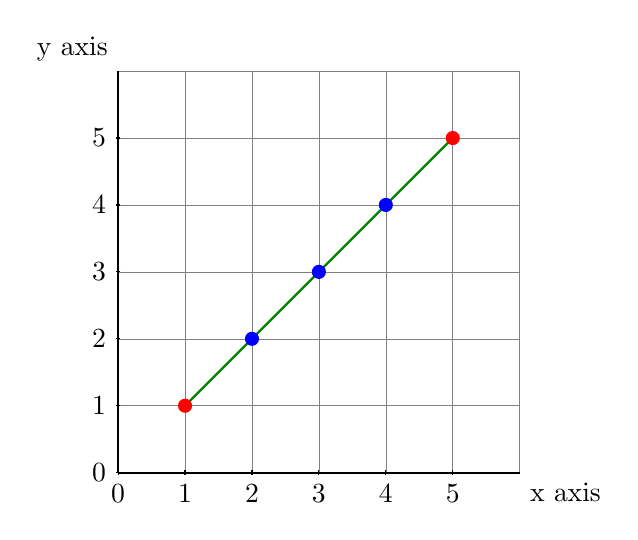
\begin{tikzpicture}[scale=0.85]
    \draw[step=1cm,gray,very thin] (0,0) grid (6,6);

    \draw[thick, -] (0,0) -- (6,0) node[anchor=north west] {x axis};
    \draw[thick, -] (0,0) -- (0,6) node[anchor=south east] {y axis};
    
    \foreach \x in {0,1,2,3,4,5}
       \draw (\x cm,1pt) -- (\x cm,-1pt) node[anchor=north] {$\x$};
    \foreach \y in {0,1,2,3,4,5}
        \draw (1pt,\y cm) -- (-1pt,\y cm) node[anchor=east] {$\y$};

    \draw[green!50!black, thick, -] (1,1) -- (5,5);

    \fill[fill=red] (1,1) circle (3pt);
    \fill[fill=red] (5,5) circle (3pt);

    \fill[fill=blue] (2,2) circle (3pt);
    \fill[fill=blue] (3,3) circle (3pt);
    \fill[fill=blue] (4,4) circle (3pt);
\end{tikzpicture}